\section{Logical view}

\textit{In de logische weergave wordt de architectuur benaderd vanuit het oogpunt van de eindgebruiker. Hierin komen de functionaliteiten van de verschillende componenten aan bod om de functionaliteit te ondersteunen.}

\begin{figure}[h]
  \centering
  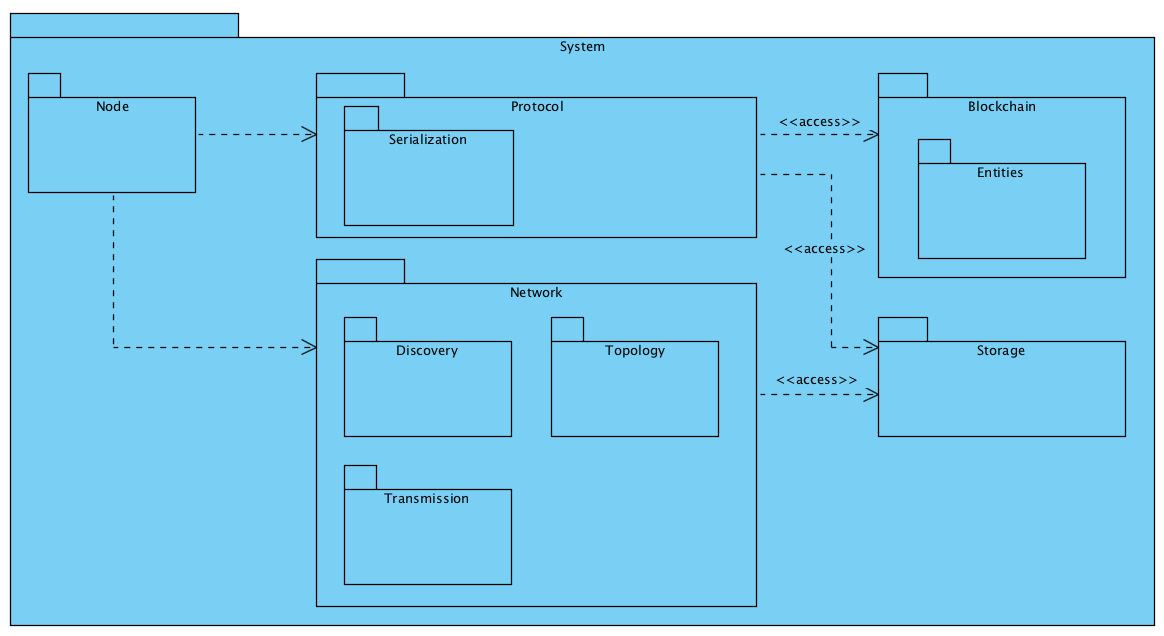
\includegraphics[width=1\textwidth]{package_diagram}
  \caption{Overzicht van het systeem}
  \label{diagram:package}
\end{figure}

In fig. \ref{diagram:package} is een overzicht te zien van de verschillende onderdelen van het systeem. De node is het startpunt van het systeem en maakt gebruik van een protocol specificatie om entiteiten uit de Blockchain op te maken in berichten die geschikt zijn voor het geïmplementeerde protocol. 

Daarnaast maakt het gebruik van de netwerk specificatie om het toe te treden, de topologie te creëren en berichten die gemaakt zijn door het protocol te versturen.

Op de volgende pagina's zijn de verschillende componenten in detail gemodelleerd.

\newpage
\begin{figure}[h]
  \centering
  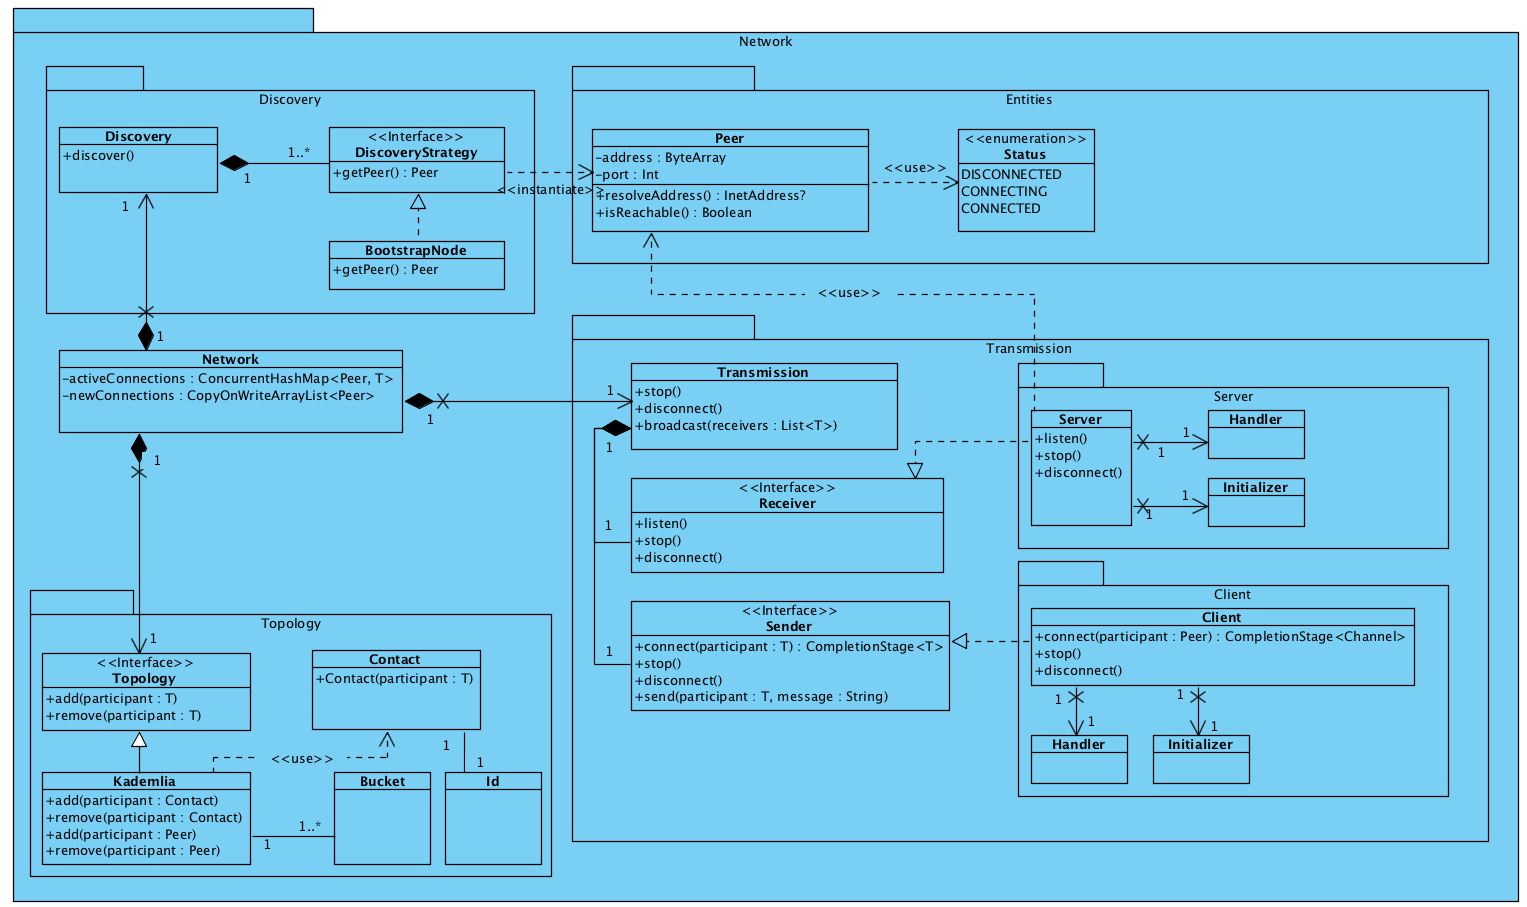
\includegraphics[width=1\textwidth]{network}
  \caption{Gedetailleerd overzicht van het Network component}
  \label{diagram:network}
\end{figure}

In fig. \ref{diagram:network} is een gedetailleerd overzicht te van van het Network component. Het Discovery component is verantwoordelijk voor het uitvoeren van het Peer Discovery Protocol dat gebruikt wordt ten tijde van het toetreden van het netwerk. Er wordt hierbij gebruik gemaakt van een strategie, namelijk het opzoeken van een BootstrapNode. 

Het Topology component is verantwoordelijk voor de structuur van het netwerk. Dit is modulair opgebouwd zodat het makkelijk gewisseld kan worden door een andere implementatie. De default topology is het Kademlia protocol.

Het Transmission component is verantwoordelijk voor het versturen en ontvangen van berichten. Dit is opgesplitst in een \textit{Receiver} en \textit{Sender} interface zodat het niet protocol specifiek geïmplementeerd hoeft te zijn.

